\section{Motivation}

The previous chapter developed the standard feasibility and stability theory for nominal MPC.
The central result was that recursive feasibility and closed-loop stability can be guaranteed by
adding suitable terminal ingredients: a terminal set, a terminal controller, and a terminal cost
satisfying an invariance and Lyapunov decrease condition. This gives a clean theoretical
construction for regulation to the origin.\\

In practice, however, MPC is rarely used only as a regulator to the origin. The controller is
usually required to track a nonzero reference, reject disturbances, operate with measured or
estimated outputs rather than full state measurements, and remain usable even when some state
or output constraints cannot be satisfied exactly. Moreover, terminal constraints, although very
useful for theoretical guarantees, may reduce the feasible set and make the online optimization
problem more restrictive than desired.\\
This chapter discusses these practical issues. We first extend the regulation formulation to
reference tracking. The key idea is to compute a steady-state target corresponding to the desired
reference and then formulate the MPC problem in deviation variables around that target. We
then discuss offset-free tracking, where constant disturbances or model mismatch would otherwise
lead to steady-state tracking errors. Finally, we consider two ways of enlarging the practical
operating region of MPC: removing terminal constraints, and softening state or output constraints.

\section{Reference Tracking}

\subsection{From regulation to tracking}

Consider the linear discrete-time system
\[
    x(k+1) = Ax(k) + Bu(k),
\]
where \(x(k) \in \R^{n_x}\) and \(u(k) \in \R^{n_u}\). The state and input are constrained to lie in
polyhedral sets
\[
    \cX = \{x \in \R^{n_x} \mid G_x x \le h_x\}, \qquad
    \cU = \{u \in \R^{n_u} \mid G_u u \le h_u\}.
\]
The standard MPC problem studied in the previous chapters is a regulation problem: the origin
is the desired equilibrium, and the cost penalizes deviations of \(x\) and \(u\) from zero.\\
In many applications, the control goal is instead to track a nonzero output reference. Let
\[
    z(k) = Hx(k)
\]
be the controlled output, and let \(r \in \R^{n_r}\) be the desired constant reference. The tracking
objective is
\[
    z(k) = Hx(k) \longrightarrow r
    \qquad \text{as } k \to \infty .
\]
In this chapter we focus on constant references, or on piecewise constant references that change
only occasionally. Time-varying reference trajectories require additional prediction information
and will not be considered here.\\
The main conceptual question is how to convert a desired output reference \(r\) into a state-input
target for the MPC controller. For regulation to the origin, the target is already known:
\((x_s,u_s)=(0,0)\). For tracking, however, the output reference \(r\) may correspond to a
nonzero equilibrium \((x_s,u_s)\), and this equilibrium must first be computed.

\subsection{The steady-state target problem}

A target state \(x_s\) achieves the output reference if
\[
    Hx_s = r.
\]
However, this condition alone is not sufficient. The state \(x_s\) must also be a steady-state of
the system under some constant input \(u_s\). Otherwise the system could pass through \(x_s\),
but it could not remain there. Therefore the target pair \((x_s,u_s)\) must satisfy
\[
    x_s = Ax_s + Bu_s,
    \qquad
    Hx_s = r.
\]
Equivalently,
\[
    \begin{bmatrix}
        I-A & -B \\
        H   & 0
    \end{bmatrix}
    \begin{bmatrix}
        x_s \\ u_s
    \end{bmatrix}
    =
    \begin{bmatrix}
        0 \\ r
    \end{bmatrix}.
\]
This is the algebraic steady-state target condition. It says that the desired reference must be
compatible with the system dynamics and with the controlled output map.\\
In the presence of constraints, the target must also satisfy
\[
    x_s \in \cX, \qquad u_s \in \cU.
\]
If several steady-state pairs satisfy the same reference, one can select among them by solving an
optimization problem. A common choice is to choose the cheapest steady-state input:
\[
\begin{aligned}
    \min_{x_s,u_s} \quad & u_s^\top R_s u_s \\
    \text{s.t.} \quad &
    \begin{bmatrix}
        I-A & -B \\
        H   & 0
    \end{bmatrix}
    \begin{bmatrix}
        x_s \\ u_s
    \end{bmatrix}
    =
    \begin{bmatrix}
        0 \\ r
    \end{bmatrix},\\
    & x_s \in \cX,\qquad u_s \in \cU .
\end{aligned}
\]
This problem is called the steady-state target problem. It is solved before, or together with, the
MPC optimization problem.\\
If the desired reference cannot be achieved exactly, one may instead compute a reachable
steady-state whose output is as close as possible to \(r\):
\[
\begin{aligned}
    \min_{x_s,u_s} \quad & (Hx_s-r)^\top Q_s (Hx_s-r) \\
    \text{s.t.} \quad & x_s = Ax_s + Bu_s,\\
    & x_s \in \cX,\qquad u_s \in \cU .
\end{aligned}
\]
This modified target problem is useful when the requested reference lies outside the set of
admissible steady-state outputs. In that case the controller should not attempt to track an
impossible reference, but should instead track the closest feasible steady-state output according
to the chosen weighting matrix \(Q_s\).

\subsection{MPC for reference tracking}

Once a steady-state target \((x_s,u_s)\) has been computed, the MPC problem can be modified
so that the predicted trajectory is penalized relative to this target rather than relative to the
origin. A direct tracking formulation is
\[
\begin{aligned}
    \min_{U} \quad &
    \norm{z_N - Hx_s}_{P_z}^2
    +
    \sum_{i=0}^{N-1}
    \left(
        \norm{z_i-Hx_s}_{Q_z}^2
        +
        \norm{u_i-u_s}_{R}^2
    \right) \\
    \text{s.t.} \quad &
    x_{i+1}=Ax_i+Bu_i,\qquad i=0,\dots,N-1,\\
    & x_i\in\cX,\qquad u_i\in\cU,\qquad i=0,\dots,N-1,\\
    & x_0=x(k).
\end{aligned}
\]
The cost now penalizes output tracking error and deviation of the input from the steady-state
input. If the terminal ingredients are included, the terminal penalty is also centered at the
target.\\
This formulation is intuitive, but it is often more convenient to rewrite the problem in
deviation variables. Define
\[
    \Delta x := x-x_s,\qquad \Delta u := u-u_s.
\]
Because \((x_s,u_s)\) is a steady-state,
\[
    x_s = Ax_s + Bu_s.
\]
Therefore the deviation dynamics are
\[
\begin{aligned}
    \Delta x(k+1)
    &= x(k+1)-x_s \\
    &= Ax(k)+Bu(k)-(Ax_s+Bu_s)\\
    &= A(x(k)-x_s)+B(u(k)-u_s)\\
    &= A\Delta x(k)+B\Delta u(k).
\end{aligned}
\]
Thus, for a linear system, the deviation variables satisfy exactly the same system matrices
\(A\) and \(B\). This is why tracking can be viewed as a regulation problem after a change of
coordinates.\\
The constraints are shifted accordingly. Since
\[
    G_x x \le h_x
    \quad \Longleftrightarrow \quad
    G_x(\Delta x+x_s)\le h_x,
\]
the state constraint becomes
\[
    G_x\Delta x \le h_x-G_xx_s.
\]
Similarly, the input constraint becomes
\[
    G_u\Delta u \le h_u-G_u u_s.
\]
The tracking MPC problem in deviation form is therefore
\[
\begin{aligned}
    \min_{\Delta U} \quad &
    \sum_{i=0}^{N-1}
    \left(
        \Delta x_i^\top Q\Delta x_i
        +
        \Delta u_i^\top R\Delta u_i
    \right)
    +
    V_f(\Delta x_N)\\
    \text{s.t.} \quad &
    \Delta x_0 = x(k)-x_s,\\
    & \Delta x_{i+1}=A\Delta x_i+B\Delta u_i,\qquad i=0,\dots,N-1,\\
    & G_x\Delta x_i \le h_x-G_xx_s,\qquad i=0,\dots,N-1,\\
    & G_u\Delta u_i \le h_u-G_u u_s,\qquad i=0,\dots,N-1,\\
    & \Delta x_N \in \cX_f .
\end{aligned}
\]
After solving this regulation problem in deviation variables, the input applied to the plant is
\[
    u(k)=u_s+\Delta u_0^\star .
\]

\begin{theorembox}[Tracking as regulation in deviation variables]
For a linear system, tracking a steady-state target \((x_s,u_s)\) is equivalent to regulating the
deviation variables
\[
    \Delta x=x-x_s,\qquad \Delta u=u-u_s
\]
to the origin. The dynamics remain
\[
    \Delta x^+ = A\Delta x+B\Delta u,
\]
while the constraints are shifted by the target.
\end{theorembox}

\subsubsection{MPC for Tracking: Convergence}

We now discuss why the tracking MPC formulation inherits the convergence guarantees of the
regulation problem. The key observation is that, after introducing the deviation variables
\[
    \Delta x = x-x_s,\qquad \Delta u = u-u_s,
\]
the tracking problem becomes a regulation problem for the deviation dynamics
\[
    \Delta x^+ = A\Delta x+B\Delta u.
\]
Therefore, if the terminal ingredients are chosen as in the regulation case, then the same
Lyapunov and recursive-feasibility arguments can be applied to the shifted system.\\
Assume that the target steady-state is feasible, i.e.
\[
    x_s\in\cX,\qquad u_s\in\cU.
\]
Moreover, assume that the terminal cost \(V_f\), the terminal set \(\cX_f\), and the local
terminal controller
\[
    \Delta u = K\Delta x
\]
satisfy the usual regulation assumptions. Namely, the terminal set is invariant under the local
closed-loop dynamics,
\[
    (A+BK)\Delta x \in \cX_f
    \qquad \forall \Delta x\in\cX_f,
\]
and the terminal cost decreases along the terminal controller according to
\[
    V_f((A+BK)\Delta x)-V_f(\Delta x)
    \le
    -\ell(\Delta x,K\Delta x)
    \qquad \forall \Delta x\in\cX_f .
\]
These two conditions are exactly the same as in the regulation case. They guarantee that, once
the predicted deviation state reaches \(\cX_f\), the local controller can keep it inside
\(\cX_f\) while providing the required Lyapunov decrease.\\
For tracking, however, one additional issue appears. The terminal set is expressed in deviation
coordinates, but the real constraints are imposed on the original variables \(x\) and \(u\). Hence
the shifted terminal set must remain inside the original state constraints:
\[
    x_s \oplus \cX_f \subseteq \cX.
\]
Similarly, the terminal input obtained after shifting back to the original coordinates must satisfy
the input constraints:
\[
    u_s + K\Delta x \in \cU
    \qquad \forall \Delta x\in\cX_f .
\]
These two inclusions are the tracking-specific constraint-compatibility conditions. They say
that the terminal controller is not only admissible for the deviation system, but also admissible
for the original constrained system around the target \((x_s,u_s)\).\\
Under these assumptions, the proof follows the same logic as for stabilizing MPC in the
regulation case. At the next sampling instant, the previously optimal sequence can be shifted by
one step, and the missing terminal input can be appended using the local law
\(\Delta u=K\Delta x\). The invariance condition ensures that the new terminal deviation state
remains in \(\cX_f\), while the shifted constraint conditions ensure that the corresponding
original state and input remain in \(\cX\) and \(\cU\). This proves recursive feasibility.\\
The Lyapunov argument is also inherited from the regulation case. The optimal value function
of the tracking problem is a Lyapunov function for the deviation dynamics. Since the terminal
cost decreases sufficiently inside \(\cX_f\), the closed-loop deviation state converges to the
origin:
\[
    \Delta x(k)\to 0
    \qquad \text{as } k\to\infty.
\]
Returning to the original coordinates, this means
\[
    x(k)\to x_s.
\]
Consequently, since the controlled output is \(z(k)=Hx(k)\), we obtain
\[
    z(k)=Hx(k)\to Hx_s=r.
\]

\begin{theorembox}[Tracking convergence]
If the target \((x_s,u_s)\) is feasible, if the terminal set and terminal cost satisfy the usual
regulation conditions in deviation coordinates, and if
\[
    x_s\oplus\cX_f\subseteq\cX,
    \qquad
    u_s+K\Delta x\in\cU \quad \forall \Delta x\in\cX_f,
\]
then the MPC closed loop converges to the target:
\[
    x(k)\to x_s,\qquad z(k)=Hx(k)\to r.
\]
\end{theorembox}

\subsection{Terminal Sets for Tracking}

The previous convergence result shows that tracking can be treated as regulation around a
shifted steady-state target. However, this shift introduces an important practical difficulty:
the terminal set is no longer fixed at the origin, but must be placed around the target state
\(x_s\).\\
In the regulation case, the terminal constraint is simply
\[
    x_N\in\cX_f,
\]
where \(\cX_f\) is a set around the origin. In the tracking case, the terminal constraint is imposed
on the deviation state:
\[
    x_N-x_s\in\cX_f.
\]
Equivalently, in the original state coordinates,
\[
    x_N\in x_s\oplus\cX_f.
\]
Thus, the regulation terminal set is translated by the target \(x_s\).\\
The state constraints define the
admissible region \(\cX\), while the terminal set must fit inside this region after being shifted
to the desired target. If the target is well inside the constraint set, the shifted terminal set may
fit without difficulty. If, however, the target is close to the boundary of \(\cX\), then the full
terminal set may no longer fit. In that case, even though the steady-state target \(x_s\) itself is
feasible, the MPC tracking problem may become infeasible because the controller requires the
whole terminal region \(x_s\oplus\cX_f\) to be feasible.\\
This explains why the set of feasible targets can be significantly smaller than the set of
constrained steady-states. A target may satisfy
\[
    x_s\in\cX,\qquad u_s\in\cU,
\]
but still fail the stronger terminal-set condition
\[
    x_s\oplus\cX_f\subseteq\cX.
\]
The terminal set therefore gives a useful stability certificate, but it also introduces conservatism
in reference tracking.

\subsubsection{Scaling the Terminal Set}

A natural way to reduce this conservatism is to scale the terminal set. Instead of using the
same terminal set \(\cX_f\) for all targets, one uses a target-dependent scaled terminal set
\[
    \cX_f^{\mathrm{scaled}} = \alpha \cX_f,
\]
where \(\alpha\ge0\) is chosen so that the shifted set remains inside the constraints:
\[
    x_s\oplus \alpha\cX_f \subseteq \cX.
\]
The corresponding terminal input constraint must also hold:
\[
    u_s + K\Delta x \in \cU
    \qquad \forall \Delta x\in \alpha\cX_f.
\]
The reason why this scaling is admissible is that invariance is preserved under scaling for
linear closed-loop dynamics. Indeed, if \(\cX_f\) is invariant under \(A+BK\), then for every
\(\Delta x\in\cX_f\),
\[
    (A+BK)\Delta x\in\cX_f.
\]
For a scaled point \(\alpha\Delta x\), linearity gives
\[
    (A+BK)(\alpha\Delta x)
    =
    \alpha(A+BK)\Delta x
    \in
    \alpha\cX_f.
\]
Hence \(\alpha\cX_f\) is also invariant.\\
The scaling factor \(\alpha\) is therefore selected according to the available constraint margin
around the target. If \(x_s\) is far from the constraint boundary, a large value of \(\alpha\) can be
used. If \(x_s\) is close to the boundary, only a small terminal set may fit. In the limiting case,
for a target exactly on the boundary of the admissible set, one may need
\[
    \alpha=0.
\]
Then the terminal set collapses to a single point and the terminal condition becomes
\[
    x_N=x_s.
\]
This is the tracking analogue of imposing a zero terminal state constraint in the regulation
problem.

\begin{theorembox}[Target-dependent terminal sets]
In tracking MPC, the terminal set must be shifted to the target:
\[
    x_N\in x_s\oplus\cX_f.
\]
This can reduce the set of feasible references, because the whole shifted terminal set must fit
inside the constraints. Scaling the terminal set,
\[
    \cX_f^{\mathrm{scaled}}=\alpha\cX_f,
\]
reduces this conservatism while preserving invariance for linear closed-loop dynamics.
\end{theorembox}

\subsubsection{Practical Consequences}

The main practical consequence is that reference changes can affect feasibility. When the
reference changes, the target selector computes a new steady-state pair \((x_s,u_s)\). This new
target changes both the shifted constraints in deviation variables and the location of the
terminal set. Therefore, even if the MPC problem was feasible for the previous reference, it may
become infeasible for the new one.\\
This is one of the main limitations of the direct shifted-terminal-set approach to tracking.
It provides a clean extension of stabilizing MPC for regulation, but the terminal set becomes a
function of the target. In applications with frequent reference changes, this dependence can be
restrictive. More advanced tracking MPC formulations address this issue by optimizing over
artificial steady-states or by using terminal ingredients that are less directly tied to a fixed target.
\subsection{Offset-Free Tracking}

\subsubsection{Why standard tracking can have offset}

The tracking formulation developed so far assumes that the model used by the controller
describes the plant accurately. Under this assumption, if the target selector computes a
steady-state pair \((x_s,u_s)\) satisfying
\[
    x_s = Ax_s + Bu_s,
    \qquad
    Hx_s = r,
\]
then stabilizing MPC drives the state to \(x_s\) and the controlled output to \(r\).

In practice, however, the true plant is rarely described exactly by the nominal model. A
particularly important case is the presence of a constant disturbance. The plant may evolve
according to
\[
    x(k+1)=Ax(k)+Bu(k)+B_d d,
\]
with measured output
\[
    y(k)=Cx(k)+C_d d,
\]
where \(d\) is an unknown constant disturbance. Such a disturbance changes the true
steady-state relation between input, state, and output. Consequently, the nominal target
\((x_s,u_s)\) computed without accounting for \(d\) may no longer correspond to the desired
output of the real plant.\\
The result is a steady-state offset. The MPC controller may stabilize the closed-loop system, but
the output can converge to a value different from the desired set point. In other words, stability
alone does not imply zero tracking error when the model is affected by constant disturbances.

\begin{theorembox}[Objective of offset-free tracking]
The objective of offset-free tracking is to design the MPC controller so that, if the closed-loop
system is stabilized in the presence of a constant disturbance, then the controlled output still
converges to the desired set point with zero steady-state offset.
\end{theorembox}

The classical unconstrained-control solution to constant disturbances is to introduce integral
action. The integrator accumulates the tracking error and modifies the input until the steady-state
error disappears. In constrained control, however, this idea must be used carefully. Input
constraints and actuator limitations can lead to windup phenomena if integral action is added
naively. MPC therefore follows a different but related approach: the disturbance is modeled
explicitly, the state and disturbance are estimated from measurements, and the target problem is
modified using the disturbance estimate.\\
Thus the offset-free MPC architecture consists of three conceptual steps. First, augment the
prediction model with a constant disturbance model. Second, use the output measurements to
estimate both the state and the disturbance. Third, compute the steady-state target and the MPC
input using the disturbance estimate.

\subsubsection{Augmented disturbance model}

To model constant disturbances, we augment the system with an integrating disturbance state:
\[
\begin{aligned}
    x_{k+1} &= Ax_k + Bu_k + B_d d_k,\\
    d_{k+1} &= d_k,\\
    y_k &= Cx_k + C_d d_k,
\end{aligned}
\]
where \(d_k\in\R^{n_d}\). The equation
\[
    d_{k+1}=d_k
\]
encodes the assumption that the disturbance is constant over time. This does not mean that the
disturbance is known. Rather, \(d_k\) is treated as an additional state to be estimated from the
measured output.\\
In compact form, the augmented model is
\[
    \begin{bmatrix}
        x_{k+1}\\ d_{k+1}
    \end{bmatrix}
    =
    \begin{bmatrix}
        A & B_d\\
        0 & I
    \end{bmatrix}
    \begin{bmatrix}
        x_k\\ d_k
    \end{bmatrix}
    +
    \begin{bmatrix}
        B\\ 0
    \end{bmatrix}
    u_k,
\]
with output equation
\[
    y_k =
    \begin{bmatrix}
        C & C_d
    \end{bmatrix}
    \begin{bmatrix}
        x_k\\ d_k
    \end{bmatrix}.
\]
The only essential restriction on the choice of the disturbance matrices \(B_d\) and \(C_d\) is
that the augmented model must be observable, or at least detectable. In the lecture, the
following condition is used. The augmented system is observable if and only if \((A,C)\) is
observable and
\[
    \operatorname{rank}
    \begin{bmatrix}
        A-I & B_d\\
        C   & C_d
    \end{bmatrix}
    =
    n_x+n_d.
\]
This rank condition has a useful steady-state interpretation. At steady-state,
\[
    \begin{bmatrix}
        A-I & B_d\\
        C   & C_d
    \end{bmatrix}
    \begin{bmatrix}
        x_s\\ d_s
    \end{bmatrix}
    =
    \begin{bmatrix}
        0\\ y_s
    \end{bmatrix}.
\]
Thus, given a measured steady-state output \(y_s\), the disturbance \(d_s\) must be uniquely
identified by the equations. If two different disturbances could produce the same measured
steady-state output, then the estimator would not be able to distinguish them, and offset-free
compensation would not be well posed.\\
This also explains the restriction
\[
    n_d \le n_y.
\]
Since disturbances are inferred from output measurements, one cannot in general estimate more
independent constant disturbances than the number of measured outputs.

\begin{theorembox}[Observability of the augmented model]
For offset-free tracking, the disturbance model must be chosen so that the augmented state
\[
    \begin{bmatrix}x\\ d\end{bmatrix}
\]
can be reconstructed from output measurements. A standard condition is that \((A,C)\) is
observable and
\[
    \operatorname{rank}
    \begin{bmatrix}
        A-I & B_d\\
        C   & C_d
    \end{bmatrix}
    =
    n_x+n_d.
\]
In particular, the number of modeled constant disturbances cannot exceed the number of
measured outputs:
\[
    n_d\le n_y.
\]
\end{theorembox}

\subsubsection{Linear state estimation}

We now need an estimator for the augmented model. Let \(\hat x(k)\) and \(\hat d(k)\) denote
the estimates of the state and the disturbance. A linear observer can be written as
\[
\begin{bmatrix}
    \hat x(k+1)\\
    \hat d(k+1)
\end{bmatrix}
=
\begin{bmatrix}
    A & B_d\\
    0 & I
\end{bmatrix}
\begin{bmatrix}
    \hat x(k)\\
    \hat d(k)
\end{bmatrix}
+
\begin{bmatrix}
    B\\
    0
\end{bmatrix}
u(k)
+
\begin{bmatrix}
    L_x\\
    L_d
\end{bmatrix}
\left(-y(k)+C\hat x(k)+C_d\hat d(k)\right).
\]
Equivalently, the correction term is proportional to the output prediction error. The sign
convention above follows the slides: the innovation is written as
\[
    -y(k)+C\hat x(k)+C_d\hat d(k).
\]
With the opposite sign convention one would simply change the sign of the observer gain.\\
Let the estimation errors be
\[
    e_x(k)=x(k)-\hat x(k),
    \qquad
    e_d(k)=d(k)-\hat d(k).
\]
Using the plant and observer equations, the error dynamics become
\[
\begin{bmatrix}
    e_x(k+1)\\
    e_d(k+1)
\end{bmatrix}
=
\left(
\begin{bmatrix}
    A & B_d\\
    0 & I
\end{bmatrix}
+
\begin{bmatrix}
    L_x\\
    L_d
\end{bmatrix}
\begin{bmatrix}
    C & C_d
\end{bmatrix}
\right)
\begin{bmatrix}
    e_x(k)\\
    e_d(k)
\end{bmatrix}.
\]
The observer gain
\[
    L=
    \begin{bmatrix}
        L_x\\ L_d
    \end{bmatrix}
\]
is chosen so that this error system is asymptotically stable. Then
\[
    \hat x(k)\to x(k),
    \qquad
    \hat d(k)\to d,
\]
at least asymptotically in the constant-disturbance setting. In practice, this gain can be designed
by pole placement or through a Kalman filter.\\
The important point is that the estimator is not only reconstructing the plant state. It is also
identifying the constant disturbance that explains the mismatch between the nominal model and
the measured output. Once this disturbance has been estimated, it can be used to correct the
steady-state target.

\subsubsection{A steady-state property of the observer}

The previous observer has a crucial steady-state property. Suppose the observer is
asymptotically stable, and suppose that the number of outputs equals the number of modeled
constant disturbances:
\[
    n_y=n_d.
\]
At steady-state, the observer estimates satisfy
\[
    \begin{bmatrix}
        A-I & B\\
        C   & 0
    \end{bmatrix}
    \begin{bmatrix}
        \hat x_\infty\\
        u_\infty
    \end{bmatrix}
    =
    \begin{bmatrix}
        -B_d\hat d_\infty\\
        y_\infty-C_d\hat d_\infty
    \end{bmatrix}.
\]
This relation says that the estimated state and disturbance are consistent with the steady-state
input and the measured steady-state output. In particular, the observer output satisfies
\[
    C\hat x_\infty + C_d\hat d_\infty = y_\infty.
\]
Thus, at steady-state, the observer output tracks the measured output without offset.

\begin{theorembox}[Observer steady-state property]
Suppose the augmented observer is asymptotically stable and \(n_y=n_d\). Then, at
steady-state, the estimated output satisfies
\[
    C\hat x_\infty+C_d\hat d_\infty = y_\infty.
\]
Thus the observer reproduces the measured output at steady-state without offset.
\end{theorembox}

\subsubsection{Disturbance-aware target problem}

The control objective is now to track a constant reference
\[
    z(k)=Hy(k)\to r.
\]
Because the measured output is affected by the disturbance, the steady-state target equations
must be modified. If the current disturbance estimate is \(\hat d\), then the target pair
\((x_s,u_s)\) should satisfy
\[
    x_s = Ax_s + Bu_s + B_d\hat d,
\]
and
\[
    z_s = H(Cx_s+C_d\hat d)=r.
\]
The first equation modifies the steady-state condition for the state evolution. The second
modifies the target condition for the controlled variables, because the controlled output depends
on the measured output and hence also on the disturbance.\\
Equivalently, the disturbance-aware target condition is
\[
    \begin{bmatrix}
        A-I & B\\
        HC  & 0
    \end{bmatrix}
    \begin{bmatrix}
        x_s\\ u_s
    \end{bmatrix}
    =
    \begin{bmatrix}
        -B_d\hat d\\
        r-HC_d\hat d
    \end{bmatrix}.
\]
This is the same target selection idea as in nominal tracking, but with a right-hand side corrected
by the disturbance estimate. The best prediction of the steady-state disturbance is the current
estimate
\[
    \hat d_\infty \approx \hat d(k).
\]
The same construction also applies to regulation by setting \(r=0\).

\subsubsection{Offset-free MPC problem}

At each sampling instant, offset-free MPC combines estimation, target selection, and predictive
control. The controller first estimates the current state and disturbance,
\[
    \hat x(k),\qquad \hat d(k).
\]
It then computes a disturbance-corrected steady-state target \((x_s,u_s)\) from the target
problem above. Finally, it solves an MPC tracking problem using the disturbance estimate:
\[
\begin{aligned}
    \min_U \quad &
    \sum_{i=0}^{N-1}
    \left(
        (x_i-x_s)^\top Q(x_i-x_s)
        +
        (u_i-u_s)^\top R(u_i-u_s)
    \right)
    +
    V_f(x_N-x_s)\\
    \text{s.t.}\quad
    & x_0=\hat x(k),\\
    & d_0=\hat d(k),\\
    & x_{i+1}=Ax_i+Bu_i+B_d d_i,\qquad i=0,\dots,N-1,\\
    & d_{i+1}=d_i,\qquad i=0,\dots,N-1,\\
    & x_i\in\cX,\qquad u_i\in\cU,\qquad i=0,\dots,N-1,\\
    & x_N-x_s\in\cX_f.
\end{aligned}
\]
Since the predicted disturbance satisfies \(d_{i+1}=d_i\), the disturbance remains equal to the
current estimate along the prediction horizon:
\[
    d_i=\hat d(k).
\]
Therefore, as in the nominal tracking case, the problem can also be rewritten in deviation
variables around the disturbance-corrected target.\\
The resulting closed-loop architecture has the same block structure shown in the slides. The
plant produces the measured output \(y\). The estimator uses \(y\) and the applied input \(u\) to
produce \(\hat x\) and \(\hat d\). The target selector uses the reference \(r\) and the disturbance
estimate \(\hat d\) to compute \((x_s,u_s)\). The MPC regulator then computes the input \(u\)
that drives the estimated state toward the corrected target.

\begin{theorembox}[Offset-free MPC algorithm]
At each sampling time:
\[
\begin{array}{ll}
\text{1.} & \text{Estimate the state and disturbance } \hat x(k),\hat d(k).\\[2mm]
\text{2.} & \text{Compute } (x_s,u_s) \text{ from the disturbance-aware target problem.}\\[2mm]
\text{3.} & \text{Solve the MPC tracking problem using } \hat x(k) \text{ and } \hat d(k).\\[2mm]
\text{4.} & \text{Apply the first optimal input } u_0^\star.
\end{array}
\]
\end{theorembox}

\subsubsection{Main result}

We state the offset-free property in the following form. Denote by
\[
    \kappa(\hat x(k),\hat d(k),r)=u_0^\star
\]
the receding-horizon control law obtained when the estimated state is \(\hat x(k)\), the estimated
disturbance is \(\hat d(k)\), and the reference is \(r\). The resulting closed-loop system is
\[
\begin{aligned}
    x(k+1) &=
    Ax(k)+B\kappa(\hat x(k),\hat d(k),r)+B_d d,\\
    \hat x(k+1) &=
    (A+L_xC)\hat x(k)
    +(B_d+L_xC_d)\hat d(k)
    +B\kappa(\hat x(k),\hat d(k),r)
    -L_x y(k),\\
    \hat d(k+1) &=
    L_dC\hat x(k)
    +(I+L_dC_d)\hat d(k)
    -L_dy(k).
\end{aligned}
\]

\begin{theorembox}[Offset-free tracking theorem]
Consider the case in which the number of modeled constant disturbances equals the number of
outputs,
\[
    n_d=n_y.
\]
Assume that the receding-horizon controller is recursively feasible and unconstrained after
some finite time \(j\), and assume that the closed-loop system converges, i.e.
\[
    \hat x(k)\to \hat x_\infty,\qquad
    \hat d(k)\to \hat d_\infty,\qquad
    y(k)\to y_\infty
    \qquad \text{as } k\to\infty.
\]
Then the controlled output converges to the reference:
\[
    z(k)=Hy(k)\to r.
\]
\end{theorembox}

The meaning of the theorem is important. Offset-free MPC does not say that disturbances
disappear. Rather, it says that if the disturbance can be consistently estimated and if the closed
loop converges, then the steady-state target is corrected in such a way that the controlled output
tracks the desired reference. The disturbance estimate is used to modify the equilibrium around
which MPC regulates.

\subsubsection{Example: double integrator}

The slides illustrate the construction on the double integrator. The first set point is \(r=0\),
while the second set point is \(r=3\). The system has one output, one input, and one modeled
constant disturbance.\\
For standard tracking, the nominal model is
\[
    x(k+1)
    =
    \begin{bmatrix}
        1 & 1\\
        0 & 1
    \end{bmatrix}x(k)
    +
    \begin{bmatrix}
        1\\
        0.5
    \end{bmatrix}u(k),
\]
with output
\[
    z(k)=y(k)=
    \begin{bmatrix}
        1 & 0
    \end{bmatrix}x(k),
\]
and constraints
\[
    -0.5\le u(k)\le 0.5,
    \qquad
    -5\le y(k)\le 5.
\]
The nominal target condition is
\[
    \begin{bmatrix}
        I-A & -B\\
        C   & 0
    \end{bmatrix}
    \begin{bmatrix}
        x_s\\ u_s
    \end{bmatrix}
    =
    \begin{bmatrix}
        0\\ r
    \end{bmatrix}.
\]
For offset-free tracking, the model is augmented with a constant disturbance:
\[
    x(k+1)
    =
    \begin{bmatrix}
        1 & 1\\
        0 & 1
    \end{bmatrix}x(k)
    +
    \begin{bmatrix}
        1\\
        0.5
    \end{bmatrix}u(k)
    +
    \begin{bmatrix}
        1\\
        1
    \end{bmatrix}d(k),
\]
with the same measured output
\[
    z(k)=y(k)=
    \begin{bmatrix}
        1 & 0
    \end{bmatrix}x(k).
\]
The augmented observability condition requires
\[
    \begin{bmatrix}
        I-A & -B_d\\
        C   & 0
    \end{bmatrix}
\]
to have full column rank. The target condition becomes
\[
    \begin{bmatrix}
        I-A & -B\\
        C   & 0
    \end{bmatrix}
    \begin{bmatrix}
        x_s\\ u_s
    \end{bmatrix}
    =
    \begin{bmatrix}
        B_d\hat d\\
        r-C_d\hat d
    \end{bmatrix}.
\]
Figure~\ref{fig:offset_free_tracking_example} shows the qualitative difference between standard
tracking and offset-free tracking. In the standard case, the controller reacts to the reference
change but converges with a steady-state offset because the constant disturbance is not accounted
for in the target selection. In the offset-free case, the disturbance estimate modifies the target,
and the output converges to the desired set point without offset.

\begin{figure}[htbp]
    \centering
    \begin{subfigure}[b]{0.48\textwidth}
        \centering
        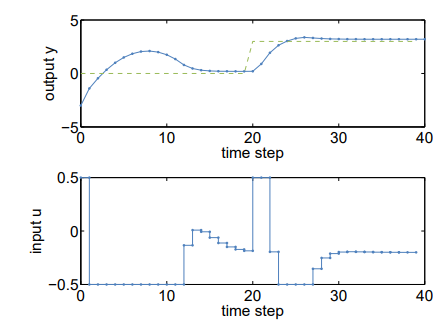
\includegraphics[width=\textwidth]{images/standard_tracking_offset_example.png}
        \caption{Standard tracking.}
        \label{fig:standard_tracking_offset_example}
    \end{subfigure}
    \hfill
    \begin{subfigure}[b]{0.48\textwidth}
        \centering
        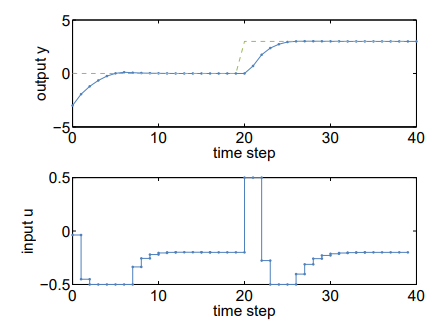
\includegraphics[width=\textwidth]{images/offset_free_tracking_example.png}
        \caption{Offset-free tracking.}
        \label{fig:offset_free_tracking_example_only}
    \end{subfigure}
    \caption{Comparison between standard tracking and offset-free tracking for the disturbed
    double integrator. Standard tracking stabilizes the system but exhibits a steady-state offset.
    Offset-free tracking estimates the constant disturbance and modifies the target condition,
    so that the output converges to the desired reference.}
    \label{fig:offset_free_tracking_example}
\end{figure}

\subsubsection{Summary of offset-free control}

Offset-free MPC can be summarized as follows. A constant disturbance is included in the model
through integrating disturbance dynamics. The output measurements are then used to estimate
both the state and the disturbance, for example by a linear observer or a Kalman filter. The
steady-state target problem is modified using the disturbance estimate, so that the target accounts
for the effect of the disturbance on both the state equation and the controlled variables. Finally,
the MPC problem is solved for regulation or tracking around this corrected target.\\
The main result is that, if the number of disturbance states equals the number of outputs, if the
target steady-state problem is feasible and no constraints are active at steady-state, and if the
closed-loop system converges, then the desired target is achieved without offset:
\[
    z(k)\to r.
\]

\begin{theorembox}[Offset-free control: main message]
Standard tracking MPC may converge with a steady-state error when constant disturbances or
model mismatch are present. Offset-free MPC removes this error by estimating the disturbance
and using it in the steady-state target problem. The controller is still an MPC tracking controller,
but it regulates around a disturbance-corrected equilibrium.
\end{theorembox}

\section{Enlarging the Feasible Set}

\subsection{Why terminal constraints may be conservative}

The stabilizing MPC construction from the previous chapter uses a terminal constraint
\[
    x_N\in\cX_f.
\]
This terminal constraint gives a clean proof of recursive feasibility and stability, but it may also
reduce the feasible set. Indeed, the optimization problem is feasible only from states that can be
driven into \(\cX_f\) within \(N\) steps while respecting all state and input constraints. If the
terminal set is small or if the horizon is short, this requirement can be restrictive.\\

Removing the terminal constraint generally enlarges the set of states for which the finite-horizon
optimization problem has a solution. It also reduces the number of constraints in the optimization
problem. In some cases, it avoids adding state constraints to problems that otherwise would have
only input constraints. From an implementation point of view, this can be attractive.\\
However, the price is theoretical. Without a terminal constraint, the feasible set of the MPC
problem is not automatically invariant. This means that the optimizer may choose a control
action that is feasible over the current horizon but leads to a state from which the next
optimization problem is infeasible. Thus, removing the terminal set may enlarge the one-step
feasible set, but it removes the simple certificate of recursive feasibility.

\subsection{MPC without Terminal Set}

We now consider the same stabilizing MPC idea, but without imposing the terminal constraint
\(x_N\in\cX_f\). The motivation is practical: as discussed above, the terminal constraint can
substantially reduce the set of initial states for which the optimization problem is feasible.
Removing it gives the controller more freedom and often enlarges the region in which a feasible
input sequence exists.\\
The finite-horizon MPC problem without terminal set is
\[
\begin{aligned}
    J^\star(x(k))=\min_U \quad &
    \sum_{i=0}^{N-1}\ell(x_i,u_i)+V_f(x_N)\\
    \text{s.t.}\quad &
    x_{i+1}=Ax_i+Bu_i,\qquad i=0,\dots,N-1,\\
    & x_i\in\cX,\qquad u_i\in\cU,\qquad i=0,\dots,N-1,\\
    & x_0=x(k).
\end{aligned}
\]
Compared with the stabilizing MPC formulation of the previous chapter, the constraint
\[
    x_N\in\cX_f
\]
has been removed. The terminal cost \(V_f(x_N)\) may still be present, but the optimizer is not
forced to end the prediction horizon inside the terminal invariant set.\\
Geometrically, this can lead to a larger feasible set. With a terminal constraint, the current
state must be such that the system can be driven into \(\cX_f\) in \(N\) steps while satisfying all
state and input constraints. Without the terminal constraint, it is enough to find a trajectory
that satisfies the state and input constraints over the finite prediction horizon. Therefore, the
feasible set without terminal constraint is generally larger.

\begin{figure}[htbp]
    \centering
    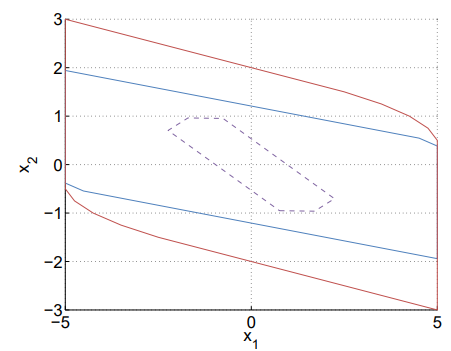
\includegraphics[width=0.5\textwidth]{images/mpc_without_terminal_feasible_set.png}
    \caption{Comparison between the feasible set with and without terminal constraint. The blue line is the feasible set with terminal constraint. The red line is the feasible set without terminal constraint. The dashed line is the terminal set.}
    \label{fig:mpc_without_terminal_feasible_set}
\end{figure}

However, this enlargement comes at a price. The feasible set without terminal constraint is not
automatically invariant. In the stabilizing construction, recursive feasibility was proved by
shifting the optimal input sequence and appending the local terminal control law
\[
    u = \kappa_f(x).
\]
This argument relied crucially on the fact that the predicted terminal state belonged to the
terminal invariant set \(\cX_f\). Without the terminal constraint, there is no guarantee that the
last predicted state lies in a region from which feasibility can be continued. Therefore, the
controller may be feasible at time \(k\), but the state reached after applying the first optimal
input may no longer admit a feasible solution at time \(k+1\).\\

The central question is then whether one can remove the terminal constraint while still retaining
stability. The answer is yes, but only under stronger and less explicit conditions. The basic idea
is that if the horizon \(N\) is sufficiently long, and if the initial state lies in a suitable subset of
the feasible region, then the optimal finite-horizon solution may naturally drive the terminal
state into the region where the terminal controller would have been valid, even though this is
not enforced as a constraint.\\
In this case, the finite-horizon solution behaves like the infinite-horizon solution over the
region of interest. The terminal constraint is no longer imposed explicitly, but the horizon is
long enough for the optimizer to ``see'' the long-term consequences of its decisions. Hence the
terminal state satisfies the desired terminal condition implicitly.

\begin{theorembox}[MPC without terminal set]
An MPC problem without terminal constraint can still be stabilizing if
\[
    x(k)
\]
belongs to a sufficiently small subset of the feasible set and the horizon \(N\) is sufficiently
large. In that case, the optimal terminal state may enter the terminal region without this being
explicitly enforced, and the finite-horizon MPC solution can coincide with the corresponding
infinite-horizon behavior on that region.
\end{theorembox}

This point is illustrated by comparing the behavior of optimal trajectories and the
resulting feasible regions. For a short horizon, the optimizer may not look far enough ahead,
and the absence of a terminal constraint can lead to poor long-term decisions. For a sufficiently
large horizon, instead, the predicted trajectory may approach the terminal region even without
being forced to do so.\\    

\begin{figure}[htbp]
    \centering
    \begin{subfigure}[b]{0.48\textwidth}
        \centering
        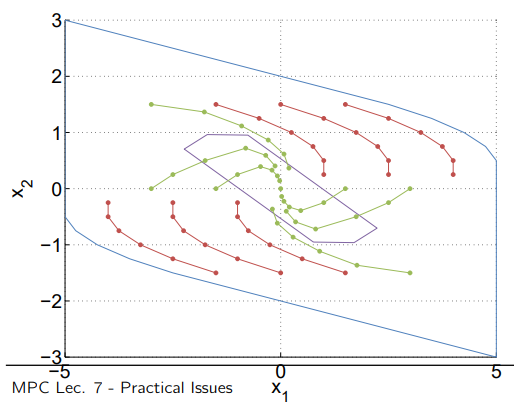
\includegraphics[width=\textwidth]{images/mpc_without_terminal_trajectories.png}
        \caption{Predicted trajectories for a sufficiently long horizon.}
        \label{fig:mpc_without_terminal_trajectories}
    \end{subfigure}
    \hfill
    \begin{subfigure}[b]{0.48\textwidth}
        \centering
        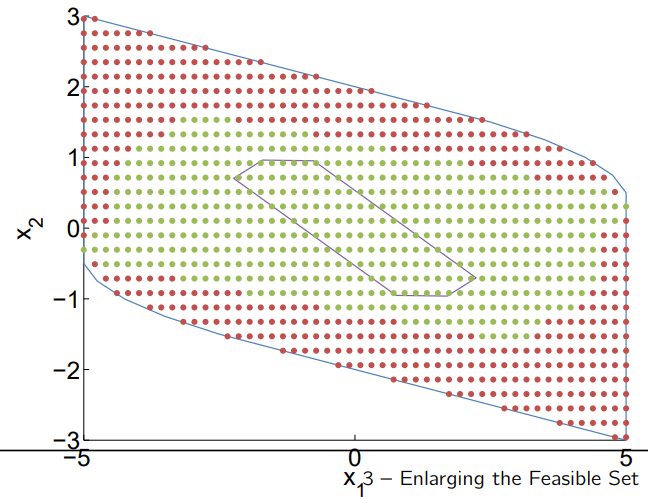
\includegraphics[width=\textwidth]{images/mpc_without_terminal_region.png}
        \caption{Region in which the terminal condition is implicitly satisfied.}
        \label{fig:mpc_without_terminal_region}
    \end{subfigure}
    \caption{MPC without terminal constraint can be stabilizing when the horizon is sufficiently
    large. The optimizer is not forced to end in \(\cX_f\), but for suitable initial conditions the
    optimal trajectory may still enter the terminal region implicitly.}
    \label{fig:mpc_without_terminal_long_horizon}
\end{figure}

The advantage of this formulation is clear: the controller may be defined on a larger feasible
set, and the optimization problem contains fewer constraints. This can be particularly attractive
when the terminal constraint introduces many additional inequalities, or when the original
problem has only input constraints and the terminal set would introduce artificial state
constraints.\\

The disadvantage is that the theoretical characterization becomes much harder. With a terminal
set, recursive feasibility and stability follow from explicit and checkable sufficient conditions:
terminal invariance and terminal Lyapunov decrease. Without a terminal set, the region of
attraction is generally difficult to compute, and the horizon length required for stability is hard
to specify a priori.\\
In practice, a common approach is therefore to choose a larger horizon and check the closed-loop
behavior by simulation or by sampling many initial conditions. This does not give the same
clean guarantee as the terminal-set construction, but it is often effective in applications. As the
horizon length increases, the region of attraction of MPC without terminal constraint tends to
approach the maximal control invariant set associated with the constraints. Intuitively, a longer
horizon gives the optimizer more information about future constraint limitations and makes the
finite-horizon problem closer to the infinite-horizon constrained control problem.

\begin{theorembox}[Practical trade-off]
The terminal constraint is a sufficient condition for recursive feasibility and stability, but it may
be conservative. Removing it can enlarge the feasible set and simplify the optimization problem,
but the region of attraction and the required horizon length become difficult to characterize.
In practice, one usually increases \(N\) and verifies stability and constraint satisfaction by
sampling or simulation.
\end{theorembox}

\subsection{Soft-Constrained MPC}

\subsubsection{Motivation for soft constraints}

We now turn to another important practical issue: what should the MPC controller do when some
constraints cannot be satisfied exactly? In the nominal formulation, constraints are hard. This
means that, if no predicted trajectory satisfies all constraints, the optimization problem becomes
infeasible and the controller is no longer defined. From a theoretical point of view this is clean,
but from an implementation point of view it is often too rigid.\\
A useful distinction must be made between input constraints and state or output constraints.
Input constraints are usually dictated by physical actuator limitations. For example, a motor
cannot provide more torque than its maximum value, and a valve cannot open beyond its physical
range. Such constraints are genuinely hard and should normally never be violated.\\

State and output constraints often have a different interpretation. They may describe desired
operating ranges, comfort bounds, product-quality limits, or safety margins. These constraints
are important, but in many applications a small and temporary violation is preferable to losing
feasibility completely. This is especially true in the presence of disturbances, measurement noise,
or model mismatch, where the measured or estimated state may move outside the nominal feasible
range.\\
This is the motivation for soft constraints. Instead of requiring selected state or output
constraints to hold exactly, one allows them to be violated by introducing slack variables. The
violation is then penalized in the objective function. In this way the controller remains defined,
but violations are made expensive.\\
The goal is therefore not to ignore constraints, but to handle violations in a controlled way.
The controller should still respect hard actuator constraints, while state or output constraints
can be softened if this is necessary to maintain feasibility.

\subsubsection{Size and duration of constraint violations}

When a state or output constraint cannot be satisfied exactly, there are two natural objectives.
One would like to minimize the duration of the violation, and one would like to minimize the
size of the violation. These two objectives are not always aligned.\\

A controller that focuses on removing the violation as quickly as possible may allow a large
temporary peak violation. Conversely, a controller that keeps the violation very small may need
more time to return fully inside the admissible region. Thus, reducing the size of the violation
can come at the cost of increasing its duration.

\begin{figure}[htbp]
    \centering
    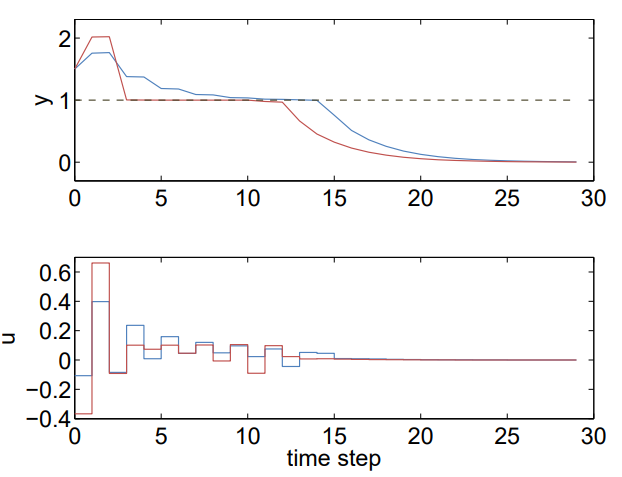
\includegraphics[width=0.6\textwidth]{images/soft_constraints_size_duration.png}
    \caption{Tradeoff between duration and size of a constraint violation. The red response
    prioritizes minimum violation time, while the blue response prioritizes minimum violation
    size.}
    \label{fig:soft_constraints_size_duration}
\end{figure}

This leads naturally to a multi-objective viewpoint. For a given system, horizon length, and
initial condition, one can imagine plotting the achievable tradeoff between violation size and
violation duration. The best operating points lie on a Pareto optimal curve. Points below this
curve cannot be attained, while points above it are inferior because another controller achieves
both smaller or equal size and smaller or equal duration.

\begin{figure}[htbp]
    \centering
    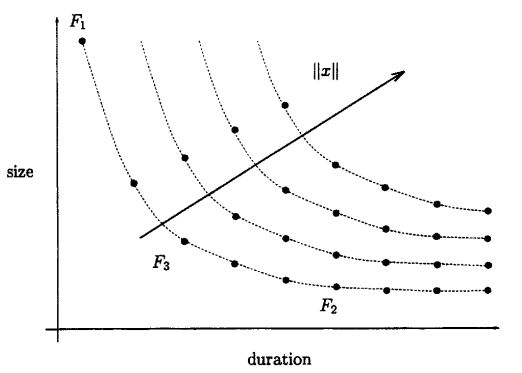
\includegraphics[width=0.5\textwidth]{images/soft_constraints_pareto_curve.png}
    \caption{Multi-objective interpretation of soft constraints. The best operation points lie on
    the Pareto optimal size-duration curve. Which point is preferable depends on the application.}
    \label{fig:soft_constraints_pareto_curve}
\end{figure}

The appropriate choice depends on the application. If a product must be discarded whenever a
quality constraint is violated, then minimizing the time spent in violation may be the most
important objective. If, instead, a large violation can trigger a shutdown or damage the process,
then minimizing the peak or total amount of violation may be more important. Soft-constrained
MPC provides a systematic way to tune this tradeoff through the penalty assigned to the slack
variables.

\subsubsection{Soft-constrained MPC formulation}

Consider again a linear prediction model
\[
    x_{i+1}=Ax_i+Bu_i.
\]
Suppose that the input constraints are kept hard:
\[
    H_u u_i \le k_u.
\]
By contrast, suppose that the state constraints
\[
    H_x x_i \le k_x
\]
are softened. To do this, introduce slack variables
\[
    \epsilon_i\in\R^p,\qquad \epsilon_i\ge0,
\]
and replace the hard state constraint by
\[
    H_xx_i \le k_x+\epsilon_i.
\]
The slack variable \(\epsilon_i\) measures how much the state constraint is relaxed at prediction
step \(i\). If the original constraint can be satisfied, the desired behavior is
\(\epsilon_i=0\). If the original constraint cannot be satisfied, then \(\epsilon_i\) allows the
optimization problem to remain feasible, but the violation is penalized in the cost.\\
The soft-constrained MPC problem can be written as
\[
\begin{aligned}
    \min_{U,\epsilon_0,\dots,\epsilon_N}\quad &
    \sum_{i=0}^{N-1}
    \left(
        x_i^\top Qx_i
        +
        u_i^\top Ru_i
        +
        \ell_\epsilon(\epsilon_i)
    \right)
    +
    x_N^\top P x_N
    +
    \ell_\epsilon(\epsilon_N)\\
    \text{s.t.}\quad &
    x_{i+1}=Ax_i+Bu_i,\qquad i=0,\dots,N-1,\\
    & H_xx_i \le k_x+\epsilon_i,\qquad i=0,\dots,N,\\
    & H_u u_i \le k_u,\qquad i=0,\dots,N-1,\\
    & \epsilon_i\ge0,\qquad i=0,\dots,N,\\
    & x_0=x(k).
\end{aligned}
\]
Here \(\ell_\epsilon(\epsilon_i)\) is the slack penalty. It determines how expensive constraint
violations are and therefore shapes the closed-loop tradeoff between violation size and violation
duration.

\begin{figure}[htbp]
    \centering
    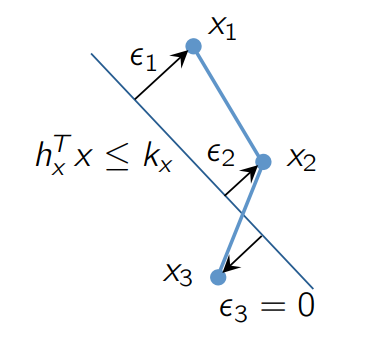
\includegraphics[width=0.45\textwidth]{images/soft_constrained_mpc_setup.png}
    \caption{Soft-constrained MPC setup. State constraints are relaxed by introducing slack
    variables \(\epsilon_i\), while input constraints remain hard. The slack variables are penalized
    in the cost.}
    \label{fig:soft_constrained_mpc_setup}
\end{figure}

A purely quadratic slack penalty has the form
\[
    \ell_\epsilon(\epsilon_i)=\epsilon_i^\top S\epsilon_i,
    \qquad S\succ0.
\]
A commonly used combined penalty adds a linear norm term:
\[
    \ell_\epsilon(\epsilon_i)
    =
    \epsilon_i^\top S\epsilon_i
    +
    v\norm{\epsilon_i}_{1/\infty}.
\]
The quadratic term is useful for tuning the magnitude of the violation and preserving a
well-posed quadratic program. The linear term is important because it can make the soft
constraint exact: if the original hard constraint is feasible, then the optimizer will choose zero
slack, provided that the linear weight is sufficiently large.

\subsubsection{Mathematical formulation of softening}

To understand the role of the slack penalty, consider the abstract constrained optimization
problem
\[
\begin{aligned}
    \min_z \quad & f(z)\\
    \text{s.t.}\quad & g(z)\le0,
\end{aligned}
\]
where, for simplicity, \(g(z)\) is scalar. The corresponding softened problem is
\[
\begin{aligned}
    \min_{z,\epsilon}\quad & f(z)+\ell_\epsilon(\epsilon)\\
    \text{s.t.}\quad & g(z)\le\epsilon,\\
    & \epsilon\ge0.
\end{aligned}
\]
The slack variable \(\epsilon\) relaxes the constraint. If \(g(z)\le0\), then the original constraint
is satisfied and one may choose \(\epsilon=0\). If \(g(z)>0\), then one can still make the
softened problem feasible by choosing \(\epsilon\ge g(z)\).

However, softening should not change the optimizer when violation is unnecessary. Therefore
we impose the following requirement.

\begin{theorembox}[Requirement on the slack penalty]
If the original hard-constrained problem has a feasible optimizer \(z^\star\), then the softened
problem should have the same optimizer and zero slack:
\[
    (z^\star,\epsilon^\star)=(z^\star,0).
\]
Thus, soft constraints should recover the original hard-constrained solution whenever the hard
constraint can be satisfied.
\end{theorembox}

This requirement is essential. Without it, the controller could decide to violate a constraint even
when a nonviolating solution exists, simply because the violation improves the performance cost.

\subsubsection{Quadratic penalty}

A natural first idea is to penalize the slack quadratically:
\[
    \ell_\epsilon(\epsilon)=s\epsilon^2,
    \qquad s>0.
\]
Although this is smooth and easy to optimize, it does not satisfy the exactness requirement in
general. The reason is that the derivative of \(s\epsilon^2\) at \(\epsilon=0\) is zero. Therefore,
an infinitesimal violation has almost no first-order cost.

To see the issue, suppose the hard constraint is
\[
    g(z) := z-z^\star \le 0,
\]
so that the feasible region is \(z\le z^\star\), and suppose that the hard-constrained optimizer is
\(z^\star\). If the objective \(f(z)\) would decrease by moving slightly to the right of \(z^\star\),
then the softened problem may prefer a point
\[
    z=z^\star+\epsilon^\star
\]
with a small but nonzero slack \(\epsilon^\star>0\). The improvement in \(f\) can dominate the
small quadratic penalty near the origin.

\begin{figure}[htbp]
    \centering
    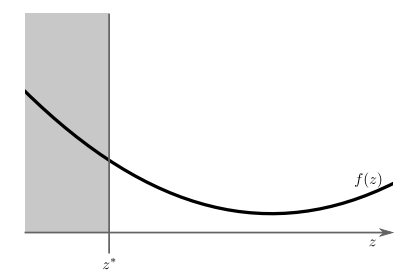
\includegraphics[width=0.45\textwidth]{images/quadratic_penalty_hard_problem.png}
    \caption{Hard-constrained problem. The grey region is the feasible set induced by
    \(g(z)=z-z^\star\le0\), and the constrained optimizer is \(z^\star\).}
    \label{fig:quadratic_penalty_hard_problem}
\end{figure}

\begin{figure}[htbp]
    \centering
    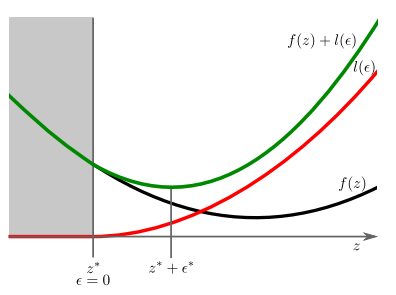
\includegraphics[width=0.45\textwidth]{images/quadratic_penalty_soft_problem.png}
    \caption{Quadratic slack penalty. Since a quadratic penalty has zero slope at the origin,
    the softened optimizer may move outside the hard feasible set and choose
    \((z^\star+\epsilon^\star,\epsilon^\star)\) instead of \((z^\star,0)\).}
    \label{fig:quadratic_penalty_soft_problem}
\end{figure}

Thus, a purely quadratic penalty is useful for tuning, but it is not an exact penalty. It may
allow constraint violation even when the hard-constrained solution is feasible.

\subsubsection{Linear penalty and exactness}

A linear penalty behaves differently:
\[
    \ell_\epsilon(\epsilon)=v\epsilon,
    \qquad v>0.
\]
Unlike the quadratic penalty, the linear penalty has nonzero slope at the origin. Therefore,
constraint violation immediately carries a first-order cost. If \(v\) is chosen sufficiently large,
then violating the constraint is more expensive than any local improvement in the original
objective \(f\), and the optimizer remains at the hard-constrained solution.\\
The precise condition is given by the optimal Lagrange multiplier of the original problem. Let
\(\lambda^\star\ge0\) be the multiplier associated with the constraint \(g(z)\le0\). Then the
linear penalty
\[
    \ell_\epsilon(\epsilon)=v\epsilon
\]
is exact if
\[
    v>\lambda^\star.
\]

\begin{theorembox}[Exact penalty function]
For the scalar constraint \(g(z)\le0\), the penalty
\[
    \ell_\epsilon(\epsilon)=v\epsilon
\]
satisfies the exactness requirement for any
\[
    v>\lambda^\star\ge0,
\]
where \(\lambda^\star\) is the optimal Lagrange multiplier of the original hard-constrained
problem.
\end{theorembox}

In practice, one often combines the exactness of the linear penalty with the tuning flexibility of
the quadratic penalty:
\[
    \ell_\epsilon(\epsilon)=v\epsilon+s\epsilon^2,
    \qquad v>\lambda^\star,\qquad s>0.
\]
For multiple constraints
\[
    g_j(z)\le0,\qquad j=1,\dots,r,
\]
with slack vector
\[
    \epsilon =
    \begin{bmatrix}
        \epsilon_1 & \cdots & \epsilon_r
    \end{bmatrix}^\top,
\]
one can use
\[
    \ell_\epsilon(\epsilon)
    =
    v\norm{\epsilon}_{1/\infty}
    +
    \epsilon^\top S\epsilon,
    \qquad S\succ0.
\]
The condition becomes
\[
    v>\norm{\lambda^\star}_D,
\]
where \(\norm{\cdot}_D\) is the dual norm of the chosen norm. In particular, the dual of
\(\norm{\cdot}_1\) is \(\norm{\cdot}_\infty\), and the dual of
\(\norm{\cdot}_\infty\) is \(\norm{\cdot}_1\).

\subsubsection{Example system}

The slides illustrate the effect of different slack penalties on a third-order nonminimum-phase
system:
\[
    x(k+1)
    =
    \begin{bmatrix}
        2 & -1.45 & 0.35\\
        1 & 0 & 0\\
        0 & 1 & 1
    \end{bmatrix}x(k)
    +
    \begin{bmatrix}
        1\\
        0\\
        0
    \end{bmatrix}u(k),
\]
with output
\[
    y(k)=
    \begin{bmatrix}
        -1 & 0 & 2
    \end{bmatrix}x(k).
\]
The output constraint is
\[
    -1\le y(k)\le 1,
\]
and the controller parameters are
\[
    Q=C^\top C,\qquad R=1,\qquad N=20.
\]
For the initial condition
\[
    x(0)=
    \begin{bmatrix}
        0.8 & 0.8 & 0.8
    \end{bmatrix}^\top,
\]
the nominal controller can satisfy the output constraint and brings the system back inside the
admissible range.

\begin{figure}[htbp]
    \centering
    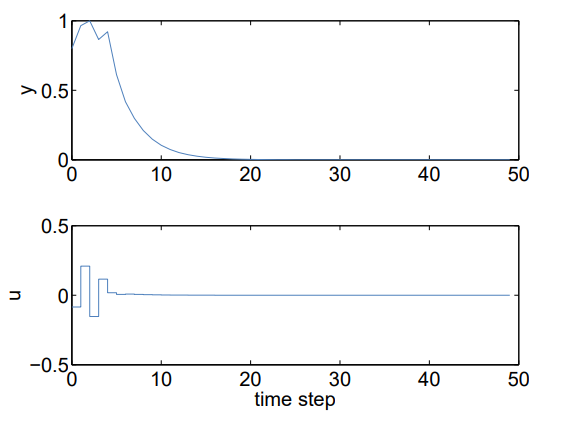
\includegraphics[width=0.6\textwidth]{images/soft_constraints_example_nominal.png}
    \caption{Third-order nonminimum-phase example used to illustrate soft constraints. The
    output constraint is \(-1\le y\le1\), with \(Q=C^\top C\), \(R=1\), and horizon \(N=20\).}
    \label{fig:soft_constraints_example_nominal}
\end{figure}

\subsubsection{Soft constraints with quadratic penalty}

We first consider a purely quadratic slack penalty:
\[
    \ell_\epsilon(\epsilon_i)=\epsilon_i^\top S\epsilon_i.
\]
This choice gives a well-posed quadratic program, because the cost remains quadratic and the
Hessian can be made positive definite. Increasing \(S\) makes the violation more expensive and
therefore hardens the soft constraint.\\
The simulation in the slides uses the initial condition
\[
    x(0)=
    \begin{bmatrix}
        1.5 & 1.5 & 1.5
    \end{bmatrix}^\top.
\]
Different values of \(S\) lead to different violation profiles. A larger \(S\) reduces the size of
the violation, but the violation tends to last longer. This is exactly the size-duration tradeoff
discussed above.

\begin{figure}[htbp]
    \centering
    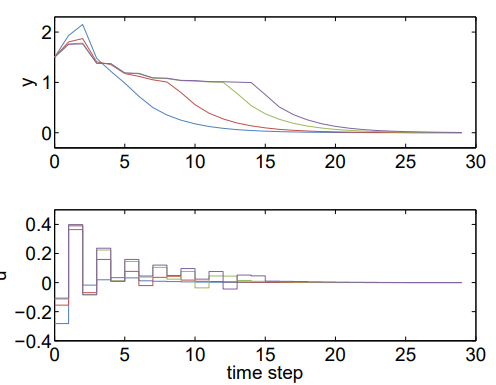
\includegraphics[width=0.6\textwidth]{images/soft_constraints_quadratic_penalty.png}
    \caption{Soft constraints with quadratic penalty. Increasing \(S\) hardens the soft
    constraint: the size of the violation is reduced, but the duration of the violation can
    increase.}
    \label{fig:soft_constraints_quadratic_penalty}
\end{figure}

Thus, the quadratic weight \(S\) is a tuning parameter. Small values of \(S\) allow larger
violations but may remove them quickly. Large values of \(S\) discourage large violations, but
can make the controller more conservative and prolong the time spent near or above the
constraint.

\subsubsection{Soft constraints with quadratic and linear penalty}

We now add a linear penalty term:
\[
    \ell_\epsilon(\epsilon_i)
    =
    \epsilon_i^\top S\epsilon_i
    +
    v\norm{\epsilon_i}_{1}.
\]
The linear term allows exact penalty behavior. If \(v\) is sufficiently large and the hard
constraint can be satisfied, the optimizer chooses zero slack. Thus, constraints are satisfied
whenever possible.\\
The slides first show a case with initial condition
\[
    x(0)=
    \begin{bmatrix}
        0.95 & 0.95 & 0.95
    \end{bmatrix}^\top,
\]
penalty norm \(1\)-norm, and quadratic weight \(S=20\). Increasing \(v\) makes violation more
expensive at the origin and pushes the controller toward satisfying the constraint whenever this
is possible.

\begin{figure}[htbp]
    \centering
    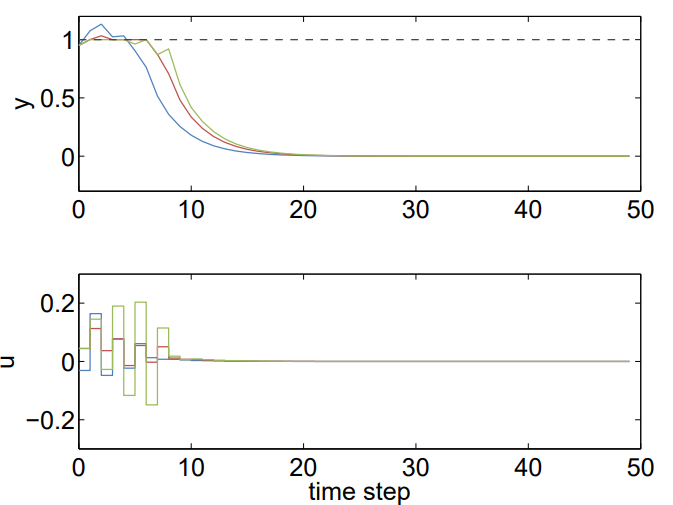
\includegraphics[width=0.6\textwidth]{images/soft_constraints_linear_quadratic_penalty_feasible.png}
    \caption{Soft constraints with combined quadratic and linear penalty for
    \(x(0)=[0.95\;0.95\;0.95]^\top\). A sufficiently large linear weight \(v\) promotes exact
    satisfaction of the constraint whenever this is possible.}
    \label{fig:soft_constraints_linear_quadratic_penalty_feasible}
\end{figure}

The second case uses the larger initial condition
\[
    x(0)=
    \begin{bmatrix}
        1.5 & 1.5 & 1.5
    \end{bmatrix}^\top,
\]
again with \(1\)-norm penalty and \(S=20\). In this case the violation cannot be avoided
completely. Increasing \(v\) changes the way the violation is distributed: larger linear penalties
tend to increase peak violations but reduce their duration. Very large values of \(v\) also make
the numerical tuning more delicate and can lead to ill-conditioned optimization problems.

\begin{figure}[htbp]
    \centering
    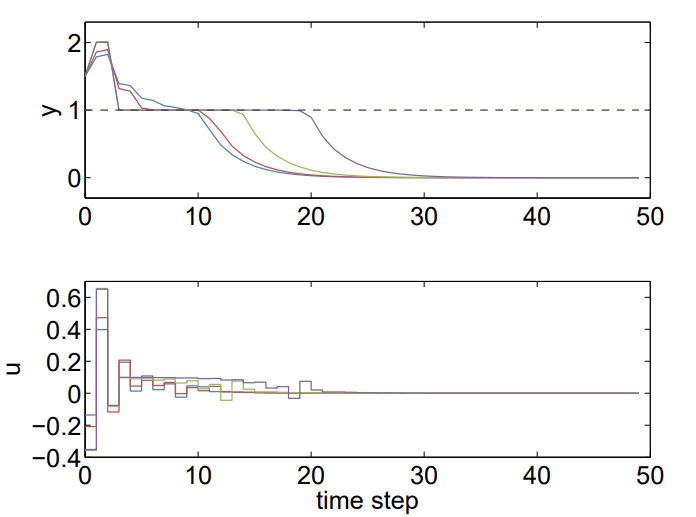
\includegraphics[width=0.6\textwidth]{images/soft_constraints_linear_quadratic_penalty_infeasible.png}
    \caption{Soft constraints with combined quadratic and linear penalty for
    \(x(0)=[1.5\;1.5\;1.5]^\top\). Increasing \(v\) tends to reduce violation duration but may
    increase peak violation and can make numerical tuning more difficult.}
    \label{fig:soft_constraints_linear_quadratic_penalty_infeasible}
\end{figure}

The role of the linear penalty is therefore twofold. It provides exactness when exact constraint
satisfaction is possible, and it influences the size-duration tradeoff when constraint violation is
unavoidable. However, \(v\) should not be chosen blindly large, since excessively large weights can
cause numerical problems and make tuning difficult.

\subsubsection{Simplification by separation of objectives}

The slides also present a useful simplification: instead of combining performance and violation
penalties in one optimization problem, one can separate the objectives into two steps.\\
First, compute the smallest constraint relaxation over the horizon:
\[
\begin{aligned}
    \epsilon^{\min}
    =
    \argmin_{u,\epsilon}\quad &
    \sum_{i=0}^{N-1}
    \left(
        \epsilon_i^\top S\epsilon_i
        +
        v^\top\epsilon_i
    \right)\\
    \text{s.t.}\quad &
    x_{i+1}=Ax_i+Bu_i,\\
    & H_xx_i\le k_x+\epsilon_i,\\
    & H_u u_i\le k_u,\\
    & \epsilon_i\ge0.
\end{aligned}
\]
Then, in a second optimization problem, optimize the controller performance subject to the
minimal relaxation already computed:
\[
\begin{aligned}
    \min_u\quad &
    \sum_{i=0}^{N-1}
    \left(
        x_i^\top Qx_i
        +
        u_i^\top Ru_i
    \right)
    +
    x_N^\top P x_N\\
    \text{s.t.}\quad &
    x_{i+1}=Ax_i+Bu_i,\\
    & H_xx_i\le k_x+\epsilon_i^{\min},\\
    & H_u u_i\le k_u.
\end{aligned}
\]
The advantage is that tuning becomes simpler. The first problem focuses only on constraint
violation, while the second problem focuses on performance given the smallest required
relaxation. In particular, constraints are satisfied whenever possible. The disadvantage is that
two optimization problems must be solved at each sampling time instead of one.


\subsubsection{Soft constraints and stability}

Soft constraints are extremely useful in practice because they recover feasibility when some state
or output constraints cannot be satisfied exactly. They also provide a systematic way to tune the
tradeoff between violation size and violation duration. For this reason, soft constraints are widely
used in industrial MPC implementations.\\
At the same time, standard soft-constrained MPC formulations do not automatically provide the
same stability guarantees as the hard-constrained stabilizing MPC construction from the previous
chapter. This issue is particularly relevant for open-loop unstable systems. By allowing state or
output constraints to be violated, the invariance-based arguments used for recursive feasibility
and stability may no longer apply directly. Additional design ingredients are needed if one wants
soft constraints together with formal stability guarantees.

\begin{theorembox}[Soft constraints: main message]
Soft constraints recover feasibility when selected constraints cannot be satisfied exactly and allow
a tunable tradeoff between violation size and violation duration. They are generally useful in
practice, but standard soft-constrained MPC does not automatically guarantee stability for
open-loop unstable systems.
\end{theorembox}

\section{Putting the Practical MPC Architecture Together}

We can now summarize the practical MPC architecture developed throughout this chapter.\\

In general, the full state is not directly measured. Therefore, the controller is typically combined
with an estimator, such as a Kalman filter, which produces an estimate \(\hat x(k)\) of the current
state. The MPC optimization is then initialized at the estimated state.\\

For reference tracking, the desired reference \(r\) is first translated into a steady-state target
\[
    (x_s,u_s).
\]
The MPC problem is then rewritten in deviation variables
\[
    \Delta x=x-x_s,\qquad \Delta u=u-u_s,
\]
so that tracking becomes regulation around the target. The terminal weight and terminal
constraint are selected as in the regulation case, but the terminal set may need to be scaled so
that the shifted terminal set fits inside the constraints.\\
To achieve offset-free tracking, the model is augmented with a constant disturbance model, and
the estimator is also augmented to estimate both \(\hat x(k)\) and \(\hat d(k)\). The target
steady-state problem is then modified using the disturbance estimate, so that the MPC regulator
tracks a disturbance-corrected equilibrium.\\
The feasible set can be enlarged by removing the terminal constraint, provided that a sufficiently
long horizon is chosen and the closed-loop behavior is checked carefully. Finally, soft constraints
can be introduced to ensure that the optimization problem remains feasible even when selected
state or output constraints cannot be satisfied exactly.
\section{Summary}

This chapter extended the nominal MPC formulation toward the issues that arise in practical
applications. The first extension was reference tracking. A desired output reference is converted
into a constrained steady-state target \((x_s,u_s)\), and the MPC problem is written in deviation
variables around this target. In this form, tracking becomes regulation, and the same terminal
cost and terminal set ideas can be used, provided that the shifted terminal set and shifted terminal
control law remain feasible.\\

The second extension was offset-free tracking. Constant disturbances and model mismatch can
cause steady-state tracking errors if the controller uses only the nominal target equation.
Offset-free MPC augments the model with integrating disturbance dynamics, estimates both the
state and the disturbance, and modifies the target problem using the disturbance estimate. Under
the appropriate convergence and feasibility assumptions, the controlled output then converges to
the desired reference without offset.\\
The third topic was enlargement of the feasible set. Terminal constraints provide a powerful
sufficient condition for recursive feasibility and stability, but they may reduce the feasible set.
Removing the terminal constraint can enlarge the operating region and simplify the optimization
problem, but the resulting feasible set is not automatically invariant and the required horizon
length is difficult to characterize.\\

Finally, we introduced soft-constrained MPC. Slack variables relax selected state or output
constraints and are penalized in the cost. This recovers feasibility when exact constraint
satisfaction is impossible and gives a tunable tradeoff between violation size and violation
duration. Quadratic penalties are smooth and easy to tune, while sufficiently large linear penalties
can be exact. Soft constraints are therefore a central practical tool, although additional care is
needed when formal stability guarantees are required.